\documentclass[uplatex]{suribt}
%\documentclass[oneside]{suribt}% 本文が * ページ以下のときに (掲示に注意)

\usepackage{hyperref}

\title{Reservoir Computer による\\カオス時系列予測と\\生体リズム研究への応用}
%\titlewidth{}% タイトル幅 (指定するときは単位つきで)
\author{久野 証}
\eauthor{Sho Kuno}% Copyright 表示で使われる
\studentid{03-210599}
\supervisor{郡 宏 教授}% 1 つ引数をとる (役職まで含めて書く)
%\supervisor{指導教員名 役職 \and 指導教員名 役職}% 複数教員の場合,\and でつなげる
\handin{2024}{2}% 提出月. 2 つ (年, 月) 引数をとる
%\keywords{キーワード1, キーワード2} % 概要の下に表示される


\begin{document}
\maketitle%%%%%%%%%%%%%%%%%%% タイトル %%%%

\frontmatter% ここから前文
\begin{abstract}%%%%%%%%%%%%% 概要 %%%%%%%%
 ここに概要を書く.
\end{abstract}

\tableofcontents%%%%%%%%%%%%% 目次 %%%%%%%%

\mainmatter% ここから本文 %%% 本文 %%%%%%%%

\chapter{はじめに}
\section{背景}
\section{本書の構成}
\clearpage
\chapter{前提知識}

\section{生体リズム研究}

\cite{koriAcceleratingRecoveryJet2017}

\cite{yamaguchiMiceGeneticallyDeficient2013a}

\section{力学系}
一般的な話.
\cite{strogatz2018nonlinear}とかを参考に一般論.


\subsection{Van Der Polモデル}

\begin{align}
    \frac{d^2 x}{d t^2}-\mu\left(1-x^2\right) \frac{d x}{d t}+x=0
\end{align}



\subsection{Rösslerモデル}
\clearpage
\section{Reservoir Computerの概要}

Reservoir ComputerはEcho State Network (ESN)の一つのモデルである.ESNはRecurrent Neural Network (RNN)の枠組みの一つで,学習の対象を出力層のみに限定することによって,従来のRNNと比較して学習コストを大幅に節約する.
ここでは,\cite{bolltExplainingSurprisingSuccess2021}に基づいて,Reservoir Computerの構造と原理について概説する.また,Reservoir Computerの理論的な背景についても,先行研究を交えながら触れる.

\textbf{構造.}
Reservoir Computerは,入力層(Input layer),レザバー層(Reservoir layer),出力層(Output/ Readout Layer)の三つの層から成る.


\begin{figure}[h]
    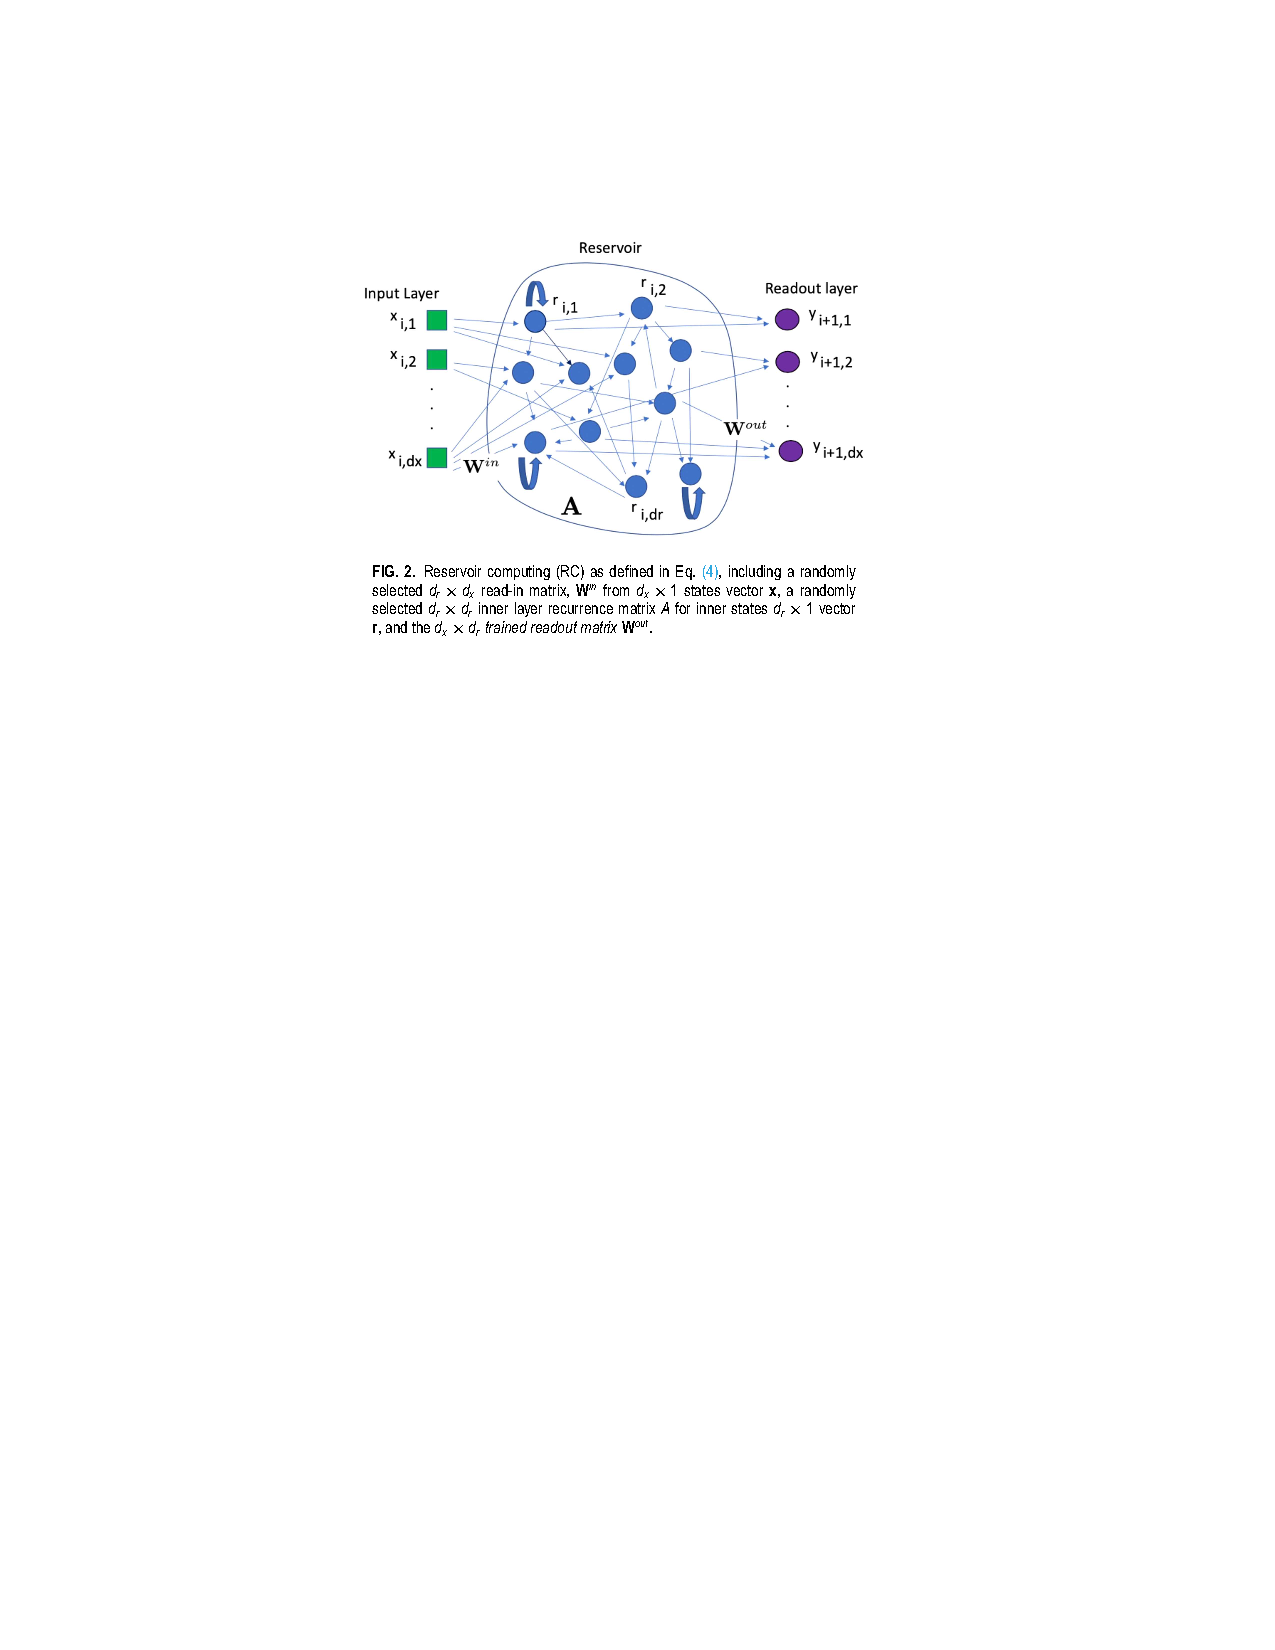
\includegraphics[width=\textwidth]{images/bollt.reservoir.pdf}
    \caption{}
\end{figure}  


\textbf{原理.}


\begin{comment}
    \begin{figure}[h]
    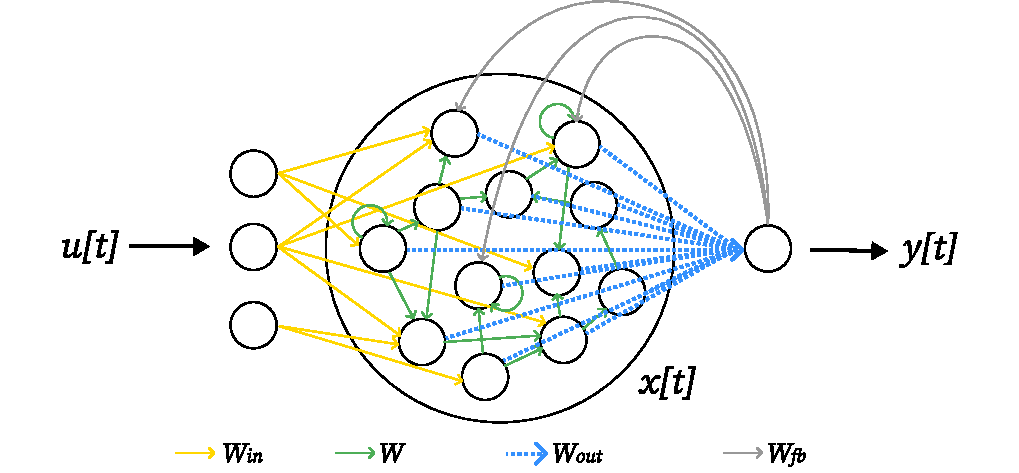
\includegraphics[width=\textwidth]{images/esn.pdf}
\end{figure}  
\begin{figure}[h]
    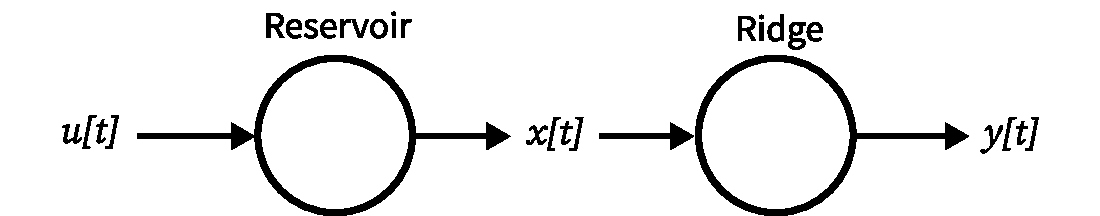
\includegraphics[width=\textwidth]{images/esn_nodes.pdf}
    \caption{}
\end{figure}  
\end{comment}


\textbf{理論的な背景.}
\cite{grigoryevaChaosCompactManifolds2021}
\cite{grigoryevaLearningStrangeAttractors2023}
\cite{berryLearningTheoryDynamical2023a}

Stochastic Inputsに対するuniversal approximationの話.
\cite{grigoryevaUniversalDiscretetimeReservoir2018}




\clearpage
\section{応用面での先行研究}


比較検討論文.二つくらいあってもいいかな.
\cite{zhangSurveyReservoirComputing2023}:Online learning/ force algorithm等に触れている.



\subsection{Y. Laiの研究内容}
本研究の直接的な先行研究として\cite{kongDigitalTwinsNonlinear2022}があるので,ここでその内容について紹介する.

\begin{figure}[h]
    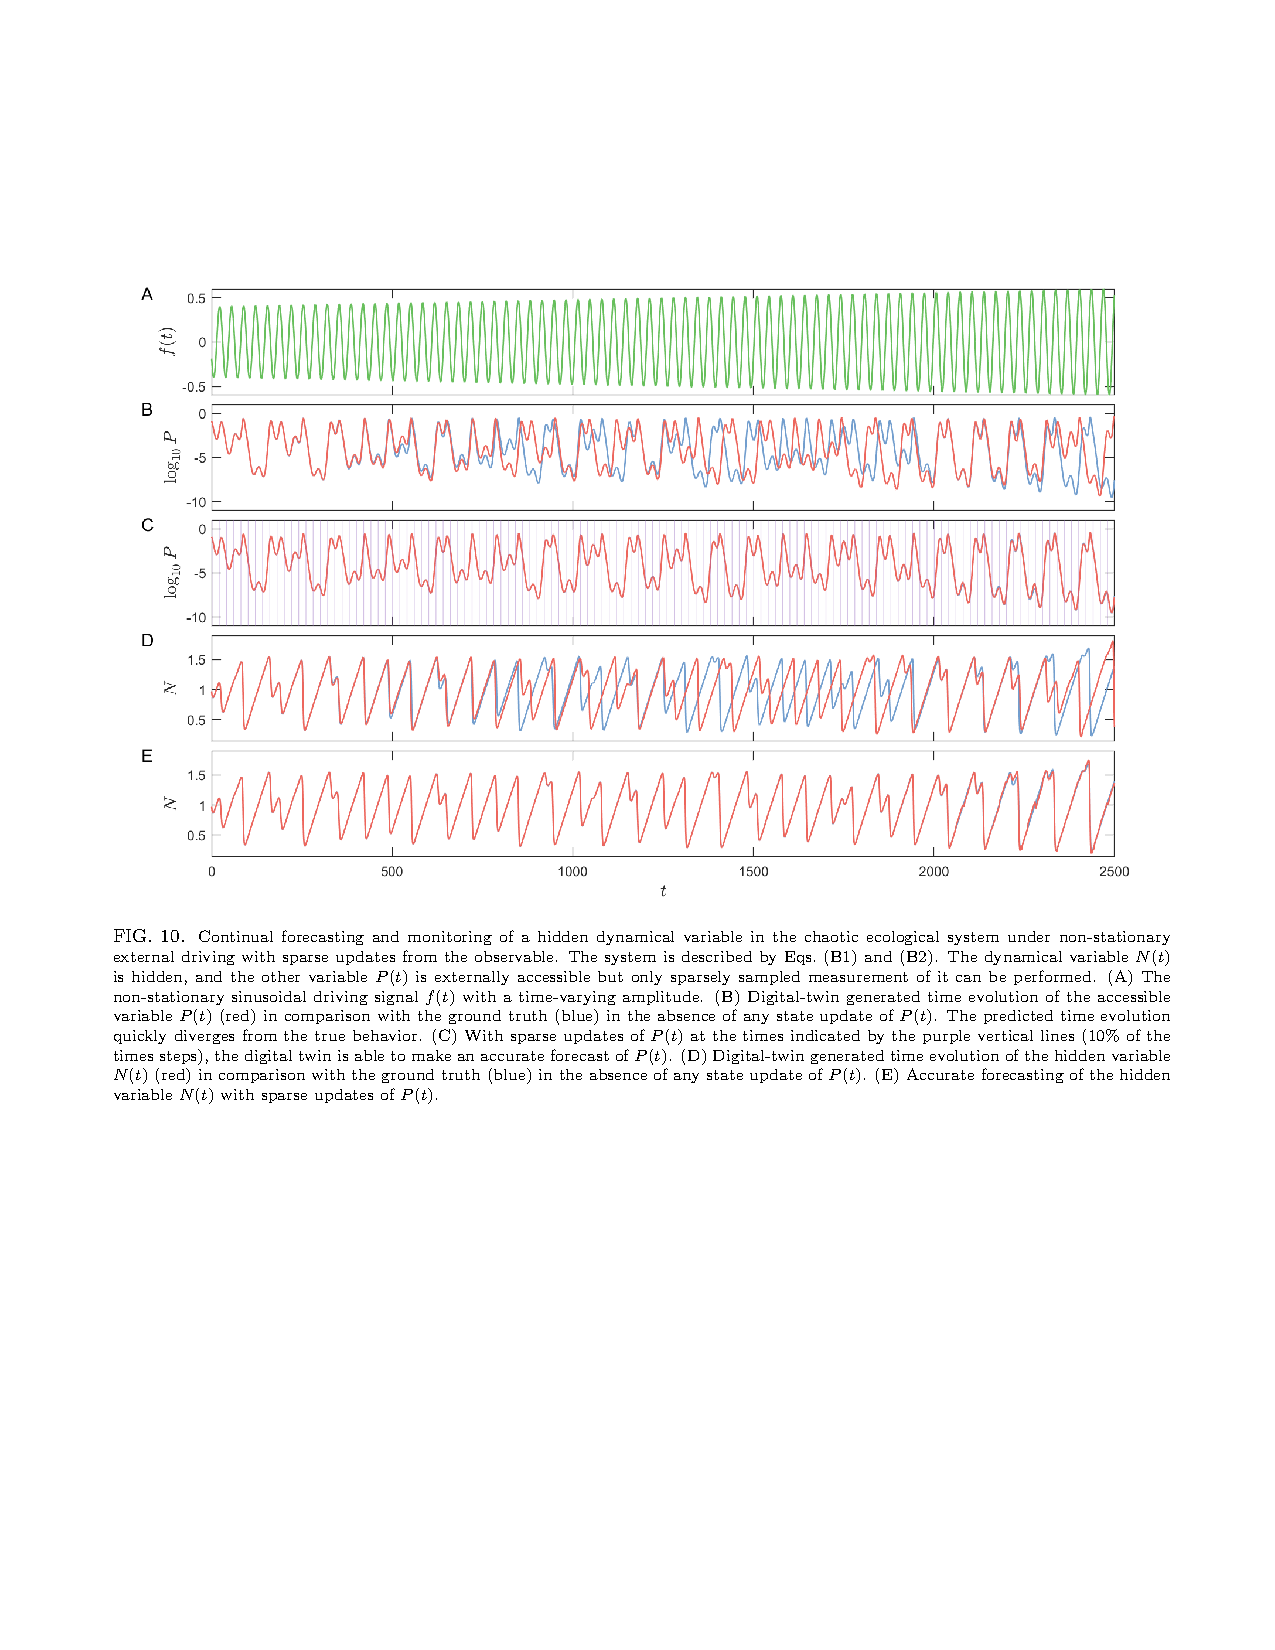
\includegraphics[width=\textwidth]{images/lai_result.pdf}
    \caption{}
\end{figure}  


\clearpage

\subsection{METHODS}
\begin{itemize}
    \item Digital twins: a recurrent RC neural network with a control
    mechanism, which requires two types of input signals:
    the observational time series for training and the con-trol signal $f(t)$ that remains in both the training and
    self-evolving phase. \begin{itemize}
        \item During the train-ing, the hidden recurrent layer is driven by both the in-
        put signal $u(t)$ and the control signal $f(t)$. 
    \end{itemize}
    \item Reservoir updating equations:
    \begin{align}
    \text{training phase: }& \mathbf{r}(t+\Delta t)=(1-\alpha) \mathbf{r}(t) + \alpha \tanh \left[\mathcal{W}_r \mathbf{r}(t)+\mathcal{W}_{\text {in }} \mathbf{u}(t)+\mathcal{W}_c f(t)\right] \\
    \text{self-evolving phase: } & \mathbf{r}(t+\Delta t)=(1-\alpha) \mathbf{r}(t) + \alpha \tanh \left[\mathcal{W}_r \mathbf{r}(t)+\mathcal{W}_{\text {in }} \mathcal{W}_{\text {out }} \mathbf{r}^{\prime}(t)+\mathcal{W}_c f(t)\right]
    \end{align}

    \item $\bold{“sense, learn, and mingle”}$: During
    the training, several trials of data are typically used un-der different driving signals so that the digital twin can
    the responses of the target sys-tem to gain the ability to extrapolate a response to a new driving signal that has never been encountered before. We input these trials of training data, i.e., a few pairs of $\mathbf{u}(t)$ and the associated $f(t)$, through the matrices $\mathcal{W}_{\text {in }}$ and $\mathcal{W}_c$ sequentially. 

    \item $\bold{validation/testing}$: the validation of the RC net-works are done with the same driving signals $f(t)$ as in
    the training data. We test driving signals $f(t)$ that are
    different from those generating the training data (e.g.,
    with different amplitude, frequency, or waveform).  

    \item $\bold{warming-up}$ During the warming-up process to initialize the RC networks prior to making the predictions, we feed randomly chosen short segments of the training time series to feed into the RC network.
    That is, no data from the target system under the testing
    driving signals $f(t)$ are required for making the predic-
    tions.
\end{itemize}


\clearpage


\subsection{RESULTS}


\chapter{議論}
\clearpage

\cite{RODRIGUES20161}

\backmatter% ここから後付
\chapter{謝辞}%%%%%%%%%%%%%%% 謝辞 %%%%%%%

%\begin{thebibliography}{}%%%% 参考文献 %%%
% \bibitem{}
%\end{thebibliography}
\bibliographystyle{unsrt}%           BibTeX を使う場合
\bibliography{reference.bib}% BibTeX を使う場合

\appendix% ここから付録 %%%%% 付録 %%%%%%%
\chapter{}
\end{document}